\documentclass[11pt,graphicx,caption,rotating]{article}
\textheight=24cm
\textwidth=18cm
\topmargin=-2cm
\oddsidemargin=0cm
\usepackage[utf8x]{inputenc}
\usepackage[activeacute,spanish]{babel}
\usepackage{amssymb,amsfonts}
\usepackage[tbtags]{amsmath}
\usepackage{pict2e}
\usepackage{float}
\usepackage[all]{xy}
\usepackage{graphics,graphicx,color,colortbl}
\usepackage{times}
\usepackage{subfigure}
\usepackage{wrapfig}
\usepackage{multicol}
\usepackage{cite}
\usepackage{url}
\usepackage[tbtags]{amsmath}
\usepackage{amsmath,amssymb,amsfonts,amsbsy}
\usepackage{bm}
\usepackage{algorithm}
\usepackage{algorithmic}
\usepackage[centerlast, small]{caption}
\usepackage[colorlinks=true, citecolor=blue, linkcolor=blue, urlcolor=blue,breaklinks=true]{hyperref}
\hyphenation{ele-men-tos he-rra-mi-en-ta cons-tru-yen trans-fe-ren-ci-a pro-pu-es-tas si-mu-lar vi-sua-li-za-cion}

\title{Taller N° 5 Modelos atómicos y Ondas de materia\\ Física Moderna}
\author{David Ricardo Martínez Hernández}
\date{17 de mayo de 2013}
\begin{document}
\maketitle

\section{Punto 1}
\noindent
Muestre y explique los niveles de energía y series espectrales del átomo de hidrógeno (Fig. 4.15 pág. 103, Libro guía: \textit{Introducción a la física Moderna, Garcia-Ewert}).\\\\
La separación entre los niveles de energía se aproxima a cero a medida que $n$ se aproxima al infinito y la energía se aproxima a cero.\\
Cero energía representa el límite entre un sistema de enlazado de un electrón y un protón y un sistema no unido. Si la energía del átomo se eleva de la del estado fundamental para cualquier energía mayor que cero, el átomo es ionizado. La energía mínima necesaria para ionizar el átomo en su estado fundamental se llama \textbf{energía de ionización}. Como puede verse a partir de la \ref{fig1}, la energía de ionización para el hidrógeno en el estado fundamental, basada en el cálculo de Bohr, es $13.6 eV$. Este hallazgo constituyó otro logro importante para la teoría de Bohr, porque la energía de ionización del hidrógeno ya se había medido fue $13.6 eV$.
\begin{figure}[H]
	\centering
		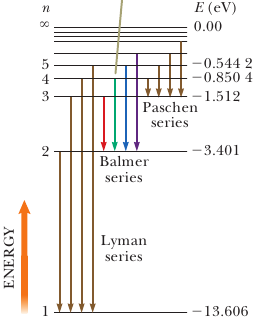
\includegraphics[scale=0.75]{line.png}
	\caption{Niveles de energía y series espectrales del átomo de hidrógeno (Tomado de \cite{serway}, página $1258$).}
	\label{fig1}
\end{figure}

\section{Punto 2}
\noindent
¿Por qué fue la serie de Balmer y no la de Lyman o Paschen la primera en ser detectada?


\section{Punto 3}
\noindent
¿Cuando en la ecuación de Rydberg para calcular longitudes de onda se hace $n_2$ tender a infinito que se obtiene?\\\\
Como la ecuación de Rydberg (ecuación (\ref{ecu30}))
\begin{equation}
 \frac{1}{\lambda_{VAC}}=R_{H}\left( {\frac{1}{{n_1^2 }} - \frac{1}{{n_2^2 }}} \right)
\label{ecu30}
\end{equation}
\noindent
donde:\\
$\lambda_{VAC}$ es la longitud de onda de la luz emitida en el vacío,\\
$R_H$ es la constante de Rydberg para el Hidrógeno, y es aproximadamente igual a $1.097 373 156 852 7*10^7\ \ m^{-1}$\\
$n_1$ y $n_2$ son enteros tal que $n_1 < n_2$.\\\\
Al hacer $n_2 \rightarrow \infty$ se obtiene la ecuación (\ref{ecu31})
\begin{eqnarray}
 \frac{1}{\lambda_{VAC}} & = & \frac{R_{H}}{n_1^2 }\label{ecu31} \\ 
 n_1^2 = 1\nonumber \\
 & = & R_H \nonumber \\
 \lambda_{VAC} & = & \frac{1}{R_H} \label{ecu32}\\
 & = & 91.1267\ \ nm\nonumber
\end{eqnarray}
\noindent
este numero es aproximadamente el \textbf{límite de la serie de Lyman}.

\section{Punto 4}
\noindent
Muestre que la energía de los niveles energéticos en el átomo de hidrógeno se puede expresar como $E_n=-hcR_H / n^2$. ¿Qué es $R_H$?\\\\
La ecuación para la mínima cantidad de energía
\begin{equation}
 E=h\nu
\label{ecu40}
\end{equation}
\begin{equation}
 E_i - E_f = h \nu
\label{ecu41}
\end{equation}
\noindent
Donde $E_i > E_f$, tomando la ecuación (\ref{ecu31}), utilizando $\nu = \frac{c}{\lambda}$ al realizar el reemplazo necesario en ellas se obtiene
\begin{eqnarray}
 E & = & \nu h \nonumber \\
 & = & -\frac{c}{\lambda} h \nonumber \\
 & = & -c \left( \frac{R_H}{n^2}\right) h \nonumber \\
 & = & -\frac{h c R_H}{n^2} \label{ecu42}
\end{eqnarray}

\section{Punto 5}
\noindent
¿Cuales serian las diferencias entre nuestro universo y uno en el cual la constante de Planck fuera $1 erg \cdotp s$?\\\\
Como $1 erg=100*10^{-9} J$. Si $h=1 erg= 100^{-9} J\cdotp s$ y no $h=6.6260755*10^{-34} J\cdotp s$, entonces si se utiliza un $\nu = 1\ \ Hz$ y se reemplaza en la ecuación (\ref{ecu40}) se obtiene
\begin{eqnarray}
 E & = & 100*10^{-9}J\cdotp s* 1s^{-1}\nonumber \\
 & = & 100*10^{-9}J \label{ecu51}
\end{eqnarray}
\noindent
es decir, la cantidad mínima de energía que puede emitirse, propagarse o ser absorbida es mucho mayor que la que se posee en este universo, la cual al ser determinada con el mismo $\nu=1\ \ Hz$ es de $E=6.6260755*10^{-34}J$, al compararlo con el resultado de la ecuación (\ref{ecu51}), $100*10^{-9}J \gg 6.626*10^{-34}J$.

\section{Punto 6}
\noindent
Demuestre que si la incertidumbre en la posición de una partícula es aproximadamente igual a su longitud de onda de De Broglie, entonces la incertidumbre en su velocidad es aproximadamente igual a su velocidad.


\section{Punto 7}
\noindent
Explique el experimento Davisson-Germer (Pág. 132 libro guía).\\\\
El experimento consistió en disparar un haz de electrones de baja energía de un cañón de electrones dirigido a una pieza de cristal de níquel en incidencia normal (es decir, perpendicular a la superficie del cristal). El experimento incluyó un cañón de electrones que consiste en un filamento caliente que libera electrones excitados térmicamente, que a continuación se acelera a través de una diferencia de potencial dándoles una cierta cantidad de energía cinética hacia el cristal de níquel. Para evitar colisiones de los electrones con otras moléculas en su camino hacia la superficie, el experimento se llevó a cabo en una cámara de vacío. Para medir el número de electrones que estaban dispersos en diferentes ángulos, un detector de electrones que puede ser movido en una trayectoria del arco sobre se utilizó el cristal. El detector fue diseñado para aceptar sólo electrones dispersados ​​elásticamente.\\
Durante el experimento se produjo un accidente y el aire entró en la cámara, produciendo una película de óxido sobre la superficie de níquel. Para quitar el óxido, Davisson y Germer calientan la muestra en un horno de alta temperatura, sin saber que este afectó a la estructura policristalina anteriormente del níquel para formar grandes zonas de cristal único con planos del cristal continuos en toda la anchura del haz de electrones.


\section{Punto 8}
\noindent
Explique detalladamente cómo funcionan el Microscopio electrónico de trasmisión (TEM) y el Microscopio electrónico de barrido (SEM).

\subsection{TEM}
\noindent
\textit{``Un microscopio electrónico de transmisión es similar en diseño a un microscopio de luz ordinaria con una diferencia clave: en lugar de utilizar la luz, utiliza electrones.\\
El uso de un tubo de rayos catódicos o filamento (una fuente para generar electrones altamente excitados) en el vacío, los electrones son acelerados hacia una determinada muestra mediante la creación de una diferencia de potencial. Una serie de imanes y de las aberturas de metal se utiliza para enfocar este vapor de electrones en un haz monocromático, que luego chocan con la muestra e interactuar dependiendo de la densidad y la carga del material. Estas interacciones se ven muy afectados por cómo se prepara la muestra''}.\footnote{\cite{page80} MIT. Transmission Electron Microscopy.  [en línea] $<$ \url{http://ocw.mit.edu/courses/biology/7-343-protein-folding-misfolding-and-human-disease-fall-2004/readings/tem.pdf} $>$, [Visitado el 11 de mayo de 2013].}

\subsubsection{Funcionamiento}
\noindent
\textit{Las partes principales de un microscopio electrónico de Transmisión son\footnote{\cite{page82} Microscopio Electrónico de Transmisión. Imágenes 3D de la nanotecnología. [en línea] $<$ \url{http://blogs.creamoselfuturo.com/nano-tecnologia/2011/03/23/microscopio-electronico-de-transmision-imagenes-3d-de-la-nanotecnologia/} $>$, [Visitado el 11 de mayo de 2013].}:
\begin{itemize}
 \item Cañón de electrones, genera el barrido electrónico que proporciona la imagen.
 \item Lentes magnéticas encargadas de enfocar el haz electrónico.
 \item Sistema de vacío es una parte muy importante del microscopio electrónico. Debido a que los electrones pueden ser desviados por las moléculas del aire, se debe hacer un vacío casi total en el interior de un microscopio de estas características. Para conseguir este flujo constante de electrones se debe operar a bajas presiones. Esto se realiza para favorecer el contraste de carga entre cátodo y tierra sin que se produzca un arco eléctrico.
 \item Placa fotográfica o pantalla fluorescente se coloca detrás del objeto a visualizar para registrar la imagen aumentada.
 \item Sistema de registro que muestra la imagen que producen los electrones, que suele ser una computadora.
\end{itemize}}

\subsection{SEM}
\noindent
\textit{``Utiliza un haz de electrones en lugar de un haz de luz para formar una imagen. Tiene una gran profundidad de campo, la cual permite que se enfoque a la vez una gran parte de la muestra. También produce imágenes de alta resolución, que significa que características espacialmente cercanas en la muestra pueden ser examinadas a una alta magnificación. La preparación de las muestras es relativamente fácil pues la mayoría de SEMs sólo requieren que estas sean conductoras''.}\footnote{\cite{page85} Wikipedia. Scanning electron microscope [en línea] $<$ \url{http://en.wikipedia.org/wiki/Scanning_electron_microscope} $>$, [Visitado el 11 de mayo de 2013].}

\subsubsection{Funcionamiento}
\noindent
\textit{``En el microscopio electrónico de barrido es necesario acelerar los electrones en un campo eléctrico, para aprovechar de esta manera su comportamiento ondulatorio, lo cual se lleva a cabo en la columna del microscopio, donde se aceleran mediante una diferencia de potencial de 1.000 a 30.000 voltios. Los electrones acelerados por un voltaje pequeño se utilizan para muestras muy sensibles, como podrían ser las muestras biológicas sin preparación adicional o muestras muy aislantes. Los voltajes elevados se utilizan para muestras metálicas, ya que éstas en general no sufren daños como las biológicas y de esta manera se aprovecha la menor longitud de onda para tener una mejor resolución. Los electrones acelerados salen del cañón, y se enfocan mediante las lentes condensadora y objetiva, cuya función es reducir la imagen del filamento, de manera que incida en la muestra un haz de electrones lo más pequeño posible (para así tener una mejor resolución). Con las bobinas deflectoras se barre este fino haz de electrones sobre la muestra, punto por punto y línea por línea.\\
Cuando el haz incide sobre la muestra, se producen muchas interacciones entre los electrones del mismo haz, y los átomos de la muestra; puede haber, por ejemplo, electrones que reboten como las bolas de billar. Por otra parte, la energía que pierden los electrones al "chocar" contra la muestra puede hacer que otros electrones salgan despedidos (electrones secundarios), y producir rayos X, electrones Auger, etc. El más común de éstos es el que detecta electrones secundarios, y es con él que se hace la mayoría de las imágenes de microscopios de barrido.\\
También podemos adquirir la señal de rayos X que se produce cuando se desprenden estos mismos de la muestra, y posteriormente hacer un análisis espectrográfico de la composición de la muestra''}.

\bibliographystyle{ieeetran}
\begin{thebibliography}{99}

\bibitem{garcia} García Castañeda, Mauricio. \& Ewert De-Geus, Jeannine.
{\em "`Introducción a la física moderna"'}.
Universidad Nacional de Colombia UNIBIBLOS, Tercera Edición, 2008.

\bibitem{serway} Serway, Raymond A. \& Jewett, John W. Jr.
{\em "`Physics for Scientists and Engineers whit Modern Physics"'}.
Brooks/Cole Cengage Learning, Eighth Edition, 2010.

\bibitem{page80} MIT. Transmission Electron Microscopy.  [en línea] $<$ \url{http://ocw.mit.edu/courses/biology/7-343-protein-folding-misfolding-and-human-disease-fall-2004/readings/tem.pdf} $>$, [Visitado el 11 de mayo de 2013].

\bibitem{page70} Wikipedia. Davisson–Germer experiment [en línea] $<$ \url{http://en.wikipedia.org/wiki/Davisson-Germer_experiment} $>$, [Visitado el 15 de mayo de 2013].

\bibitem{page82} Microscopio Electrónico de Transmisión. Imágenes 3D de la nanotecnología. [en línea] $<$ \url{http://blogs.creamoselfuturo.com/nano-tecnologia/2011/03/23/microscopio-electronico-de-transmision-imagenes-3d-de-la-nanotecnologia/} $>$, [Visitado el 11 de mayo de 2013].

\bibitem{page85} Wikipedia. Scanning electron microscope [en línea] $<$ \url{http://en.wikipedia.org/wiki/Scanning_electron_microscope} $>$, [Visitado el 11 de mayo de 2013].

\bibitem{page81} Wikipedia. Transmission electron microscopy [en línea] $<$ \url{http://en.wikipedia.org/wiki/Transmission_electron_microscopy} $>$, [Visitado el 11 de mayo de 2013].
\end{thebibliography}
\end{document}